% Chapter Template

\chapter{Experimentos}

\label{Chapter5} % Change X to a consecutive number; for referencing this chapter elsewhere, use \ref{ChapterX}

En este capítulo se detallarán las pruebas realizadas, con el objetivo de validar la solución propuesta en este trabajo. Además se comprobarán las diferentes configuraciones desarrolladas y se evaluarán sus prestaciones con los costes temporales. Estos experimentos han permitido depurar el componente para poder ajustar y mejorar la funcionalidad del mismo durante el desarrollo.

%-----------------------------------
%	SECTION Validación experimental
%-----------------------------------
\section{Validación experimental}

El entorno de pruebas utilizado ha sido siempre un entorno real, trabajando con los datos en vivo proporcionados por OpenniServer que extrae la información directamente del sensor.

Se propone en esta sección validar el componente en las diferentes fases que lo componen: detección de puntos de interés, cálculo de emparejamientos y estimación de movimiento.

\subsection{Detección de puntos de interés}



\subsection{Cálculo de emparejamientos}


\subsubsection{Posición estática}
\subsubsection{Traslación}
\subsubsection{Rotación}


\subsection{Resolución 3D}

La resolución 3D o estimación de movimiento compone el último paso que completa una iteración del sistema, por lo que en esta etapa podremos ver el resultado final del movimiento entre varios fotogramas consecutivos.

Las pruebas mostrados a continuación son realizadas con un funcionamiento normal del componente y en un tiempo determinado. El objetivo de estos experimentos es comprobar el comportamiento del sistema para los diferentes tipos de traslaciones ($x$, $y$, y $z$) y rotaciones (\textit{pitch}, \textit{yaw}, \textit{roll}).

Para estas pruebas y las siguientes se hará uso del componente con el comportamiento automático activado, repitiendo así de manera autónoma cada ciclo de estimación 3D. También se ha optado, para añadir robustez, el filtro de sobresaliencia y RANSAC.

\subsubsection{Validación de la traslación}

En la siguiente subsección se harán pruebas para comprobar como se comporta el sistema ante la traslación. Se moverá la cámara a lo largo de los tres ejes ($x$, $y$ y $z$) (Figura~\ref{fig:xyz}).

\begin{figure}[th]
\centering
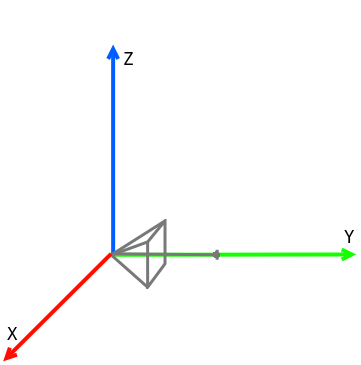
\includegraphics[scale=0.3]{Figures/xyz.png}
\decoRule
\caption[Ejes de coordenadas $x$, $y$ y $z$]{Ejes de coordenadas $x$, $y$ y $z$, con la orientación de la cámara.}
\label{fig:xyz}
\end{figure}

Para estas pruebas se va a utilizar el mismo entorno de trabajo por lo que el punto de partida será el que se muestra en la Figura~\ref{fig:init}.

\begin{figure}[th]
\centering
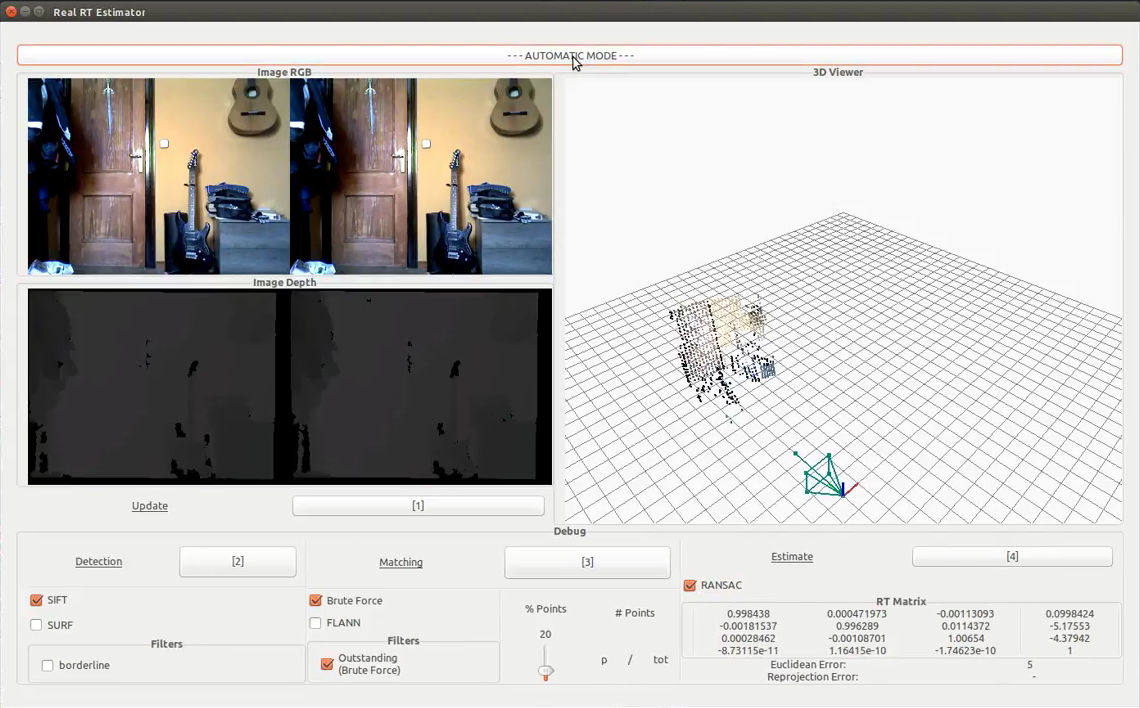
\includegraphics[scale=0.3]{Figures/tests/init.png}
\decoRule
\caption[Punto de partida para las pruebas de traslación y rotación]{Punto de partida para las pruebas realizadas.}
\label{fig:init}
\end{figure}

En la Figura~\ref{fig:axis-y} se muestra la estimación de movimiento sobre el eje $y$. El desplazamiento se ha intentado hacer lo más recto posible y el recorrido se muestra como estela en el visor 3D del componente. En ambas capturas se puede ver la ida y la vuelta recorriendo por cada una 1.5 metros aproximadamente. Después se ha vuelto a la posición de origen del movimiento.

\begin{figure}[th]
\centering
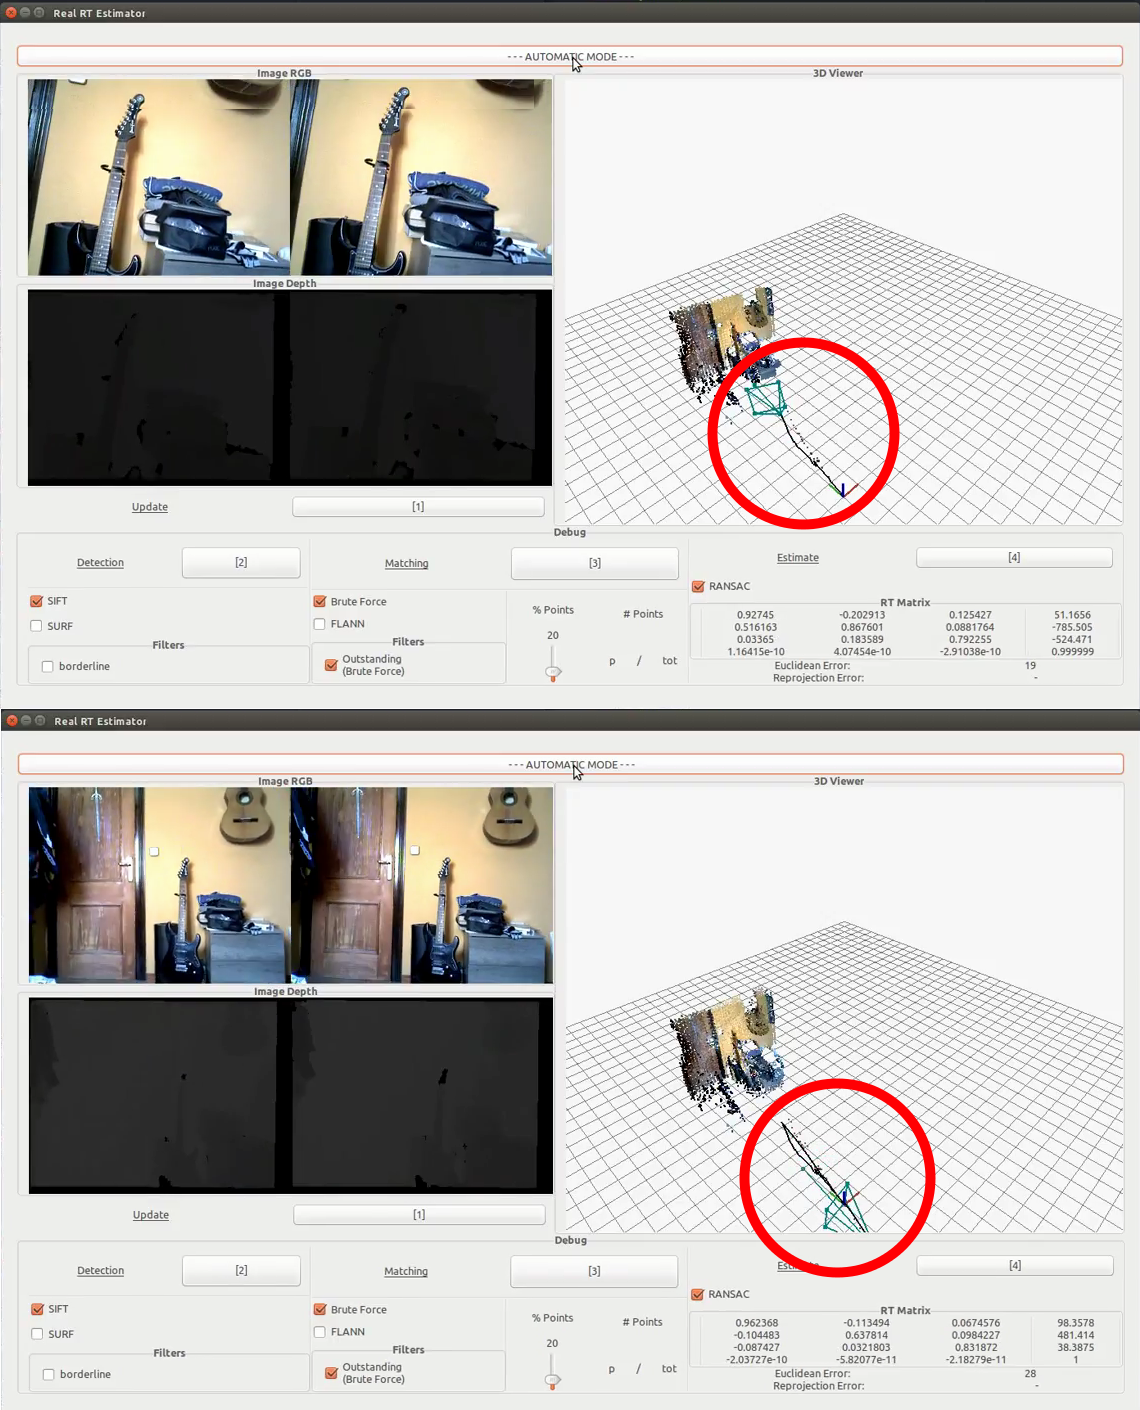
\includegraphics[scale=0.3]{Figures/tests/axis-y.png}
\decoRule
\caption[Prueba con desplazamiento en el eje $y$]{Prueba con desplazamiento en el eje $y$.}
\label{fig:axis-y}
\end{figure}

Se puede observar, después de aproximadamente 100 iteraciones, como ha afectado el error a la estimación al volver el sensor al origen.

En la Figura~\ref{fig:axis-xz} se puede ver el efecto de la traslación en los ejes $x$ y $z$ respectivamente. Se ve como el error en estos ejes es menor, percibiendo oscilaciones en su mayor parte únicamente en el eje $y$. La validación del eje $x$ se ha realizado sobre una mesa recorriendo 1 metro, por lo que no se obtiene desplazamiento en $z$. En cuanto a las pruebas del eje $z$ se aprecia un balanceo en $x$ debido al movimiento vertical de la mano ya que no ha seguido una trayectoria recta.

\begin{figure}[th]
\centering
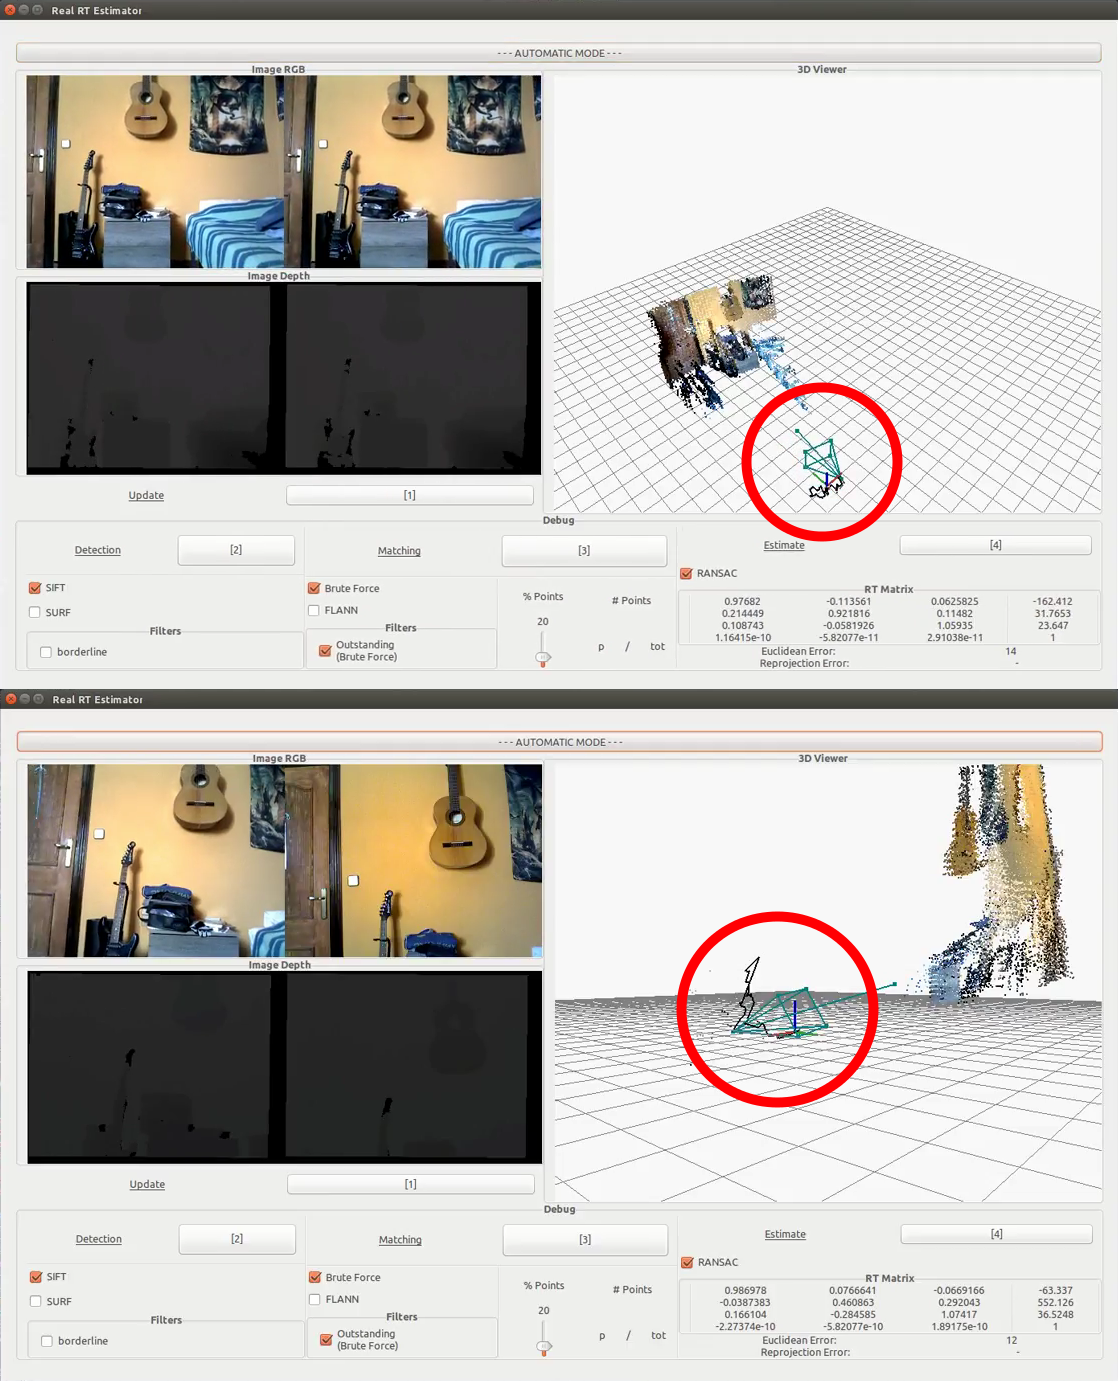
\includegraphics[scale=0.3]{Figures/tests/axis-x-z.png}
\decoRule
\caption[Prueba con desplazamiento en los ejes $x$ y $z$]{Prueba con desplazamiento en los ejes $x$ y $z$.}
\label{fig:axis-xz}
\end{figure}

Los resultados son aceptables en la estimación, no se consigue un cierre de trayectoria perfecto pero se acerca. Pensando que se ha aplicado una traslación de más de 1 metro el error final obtenido se puede medir en centímetros, acentuándose más para el eje $y$ correspondiente al perpendicular al plano imagen y el que se obtiene de la imagen de profundidad.

Como vimos en el capítulo \ref{Chapter3} la información de profundidad del sensor no es perfecta y tiene un pequeño margen de error. A parte de tener un rango de distancias óptimo establecido por el fabricante (\textit{0.8 to 3.5 m}), fuera de este rango la imagen de profundidad empieza a empeorar drásticamente y por consiguiente la estimación de movimiento.

\subsubsection{Validación de la Rotación}

Se validará ahora la rotación de sensor de los ángulos \textit{pitch}, \textit{yaw} y \textit{roll}. En la Figura~\ref{fig:p-y-r} se tiene un ejemplo gráfico de cuales son estos movimientos y a qué rotación de ejes pertenecen.

\begin{figure}[th]
\centering
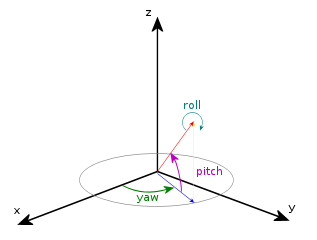
\includegraphics[scale=0.9]{Figures/pitch_yaw_roll.png}
\decoRule
\caption[Explicación gráfica del movimiento \textit{pitch}, \textit{yaw} y \textit{roll}]{Dibujo con los movimientos \textit{pitch}, \textit{yaw} y \textit{roll}.}
\label{fig:p-y-r}
\end{figure}

En la Figura~\ref{fig:pitch} se efectúa una prueba con el ángulo \textit{pitch} y se comprueba como el sistema detecta una rotación total de $90º$. Se visualiza el estado de la cámara al orientar hacia arriba el sensor y posteriormente orientándolo a nivel del suelo. 

En cuanto a la traslación se observa, sin contar con el ruido, que el eje de la cámara se mantiene fijo en el origen como es de esperar.

\begin{figure}[th]
\centering
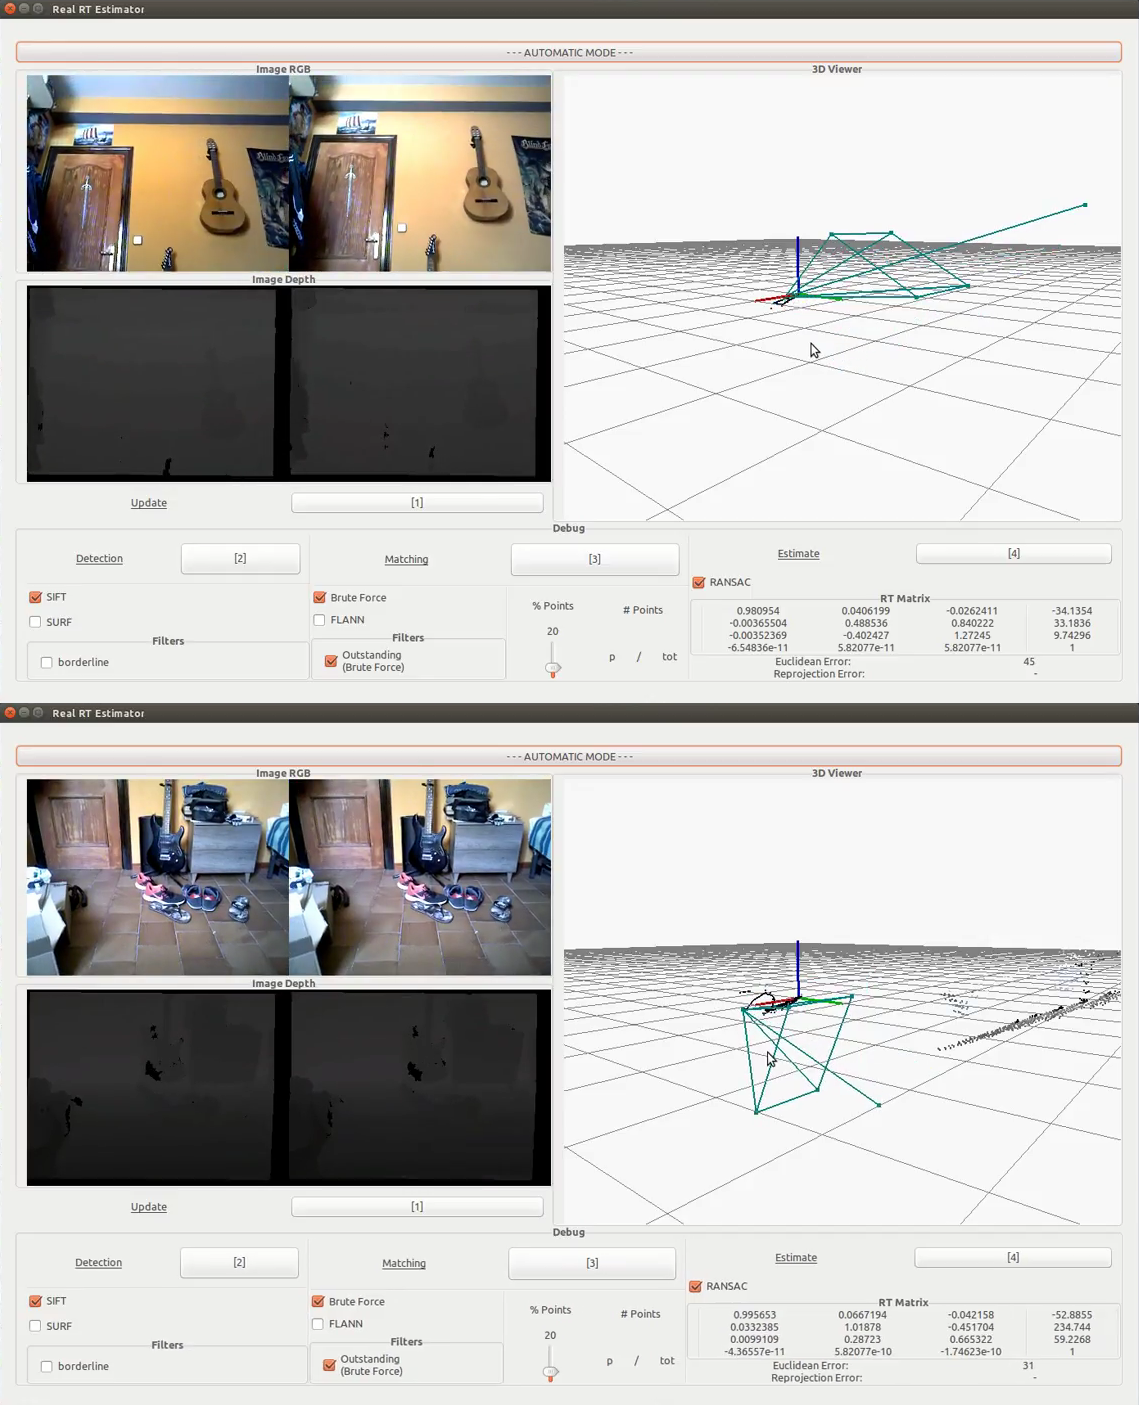
\includegraphics[scale=0.3]{Figures/tests/pitch.png}
\decoRule
\caption[Prueba con desplazamiento del ángulo \textit{pitch}]{Prueba con desplazamiento del ángulo \textit{pitch}.}
\label{fig:pitch}
\end{figure}

Para los ángulos \textit{yaw} y \textit{roll} se puede observar en la Figura~\ref{fig:yaw-roll} las pruebas realizadas. En la primera captura se observa una rotación de $45º$ sobre el eje \textit{yaw} y en la segunda sobre el eje \textit{roll}. En ambos casos el movimiento es el correcto.

\begin{figure}[th]
\centering
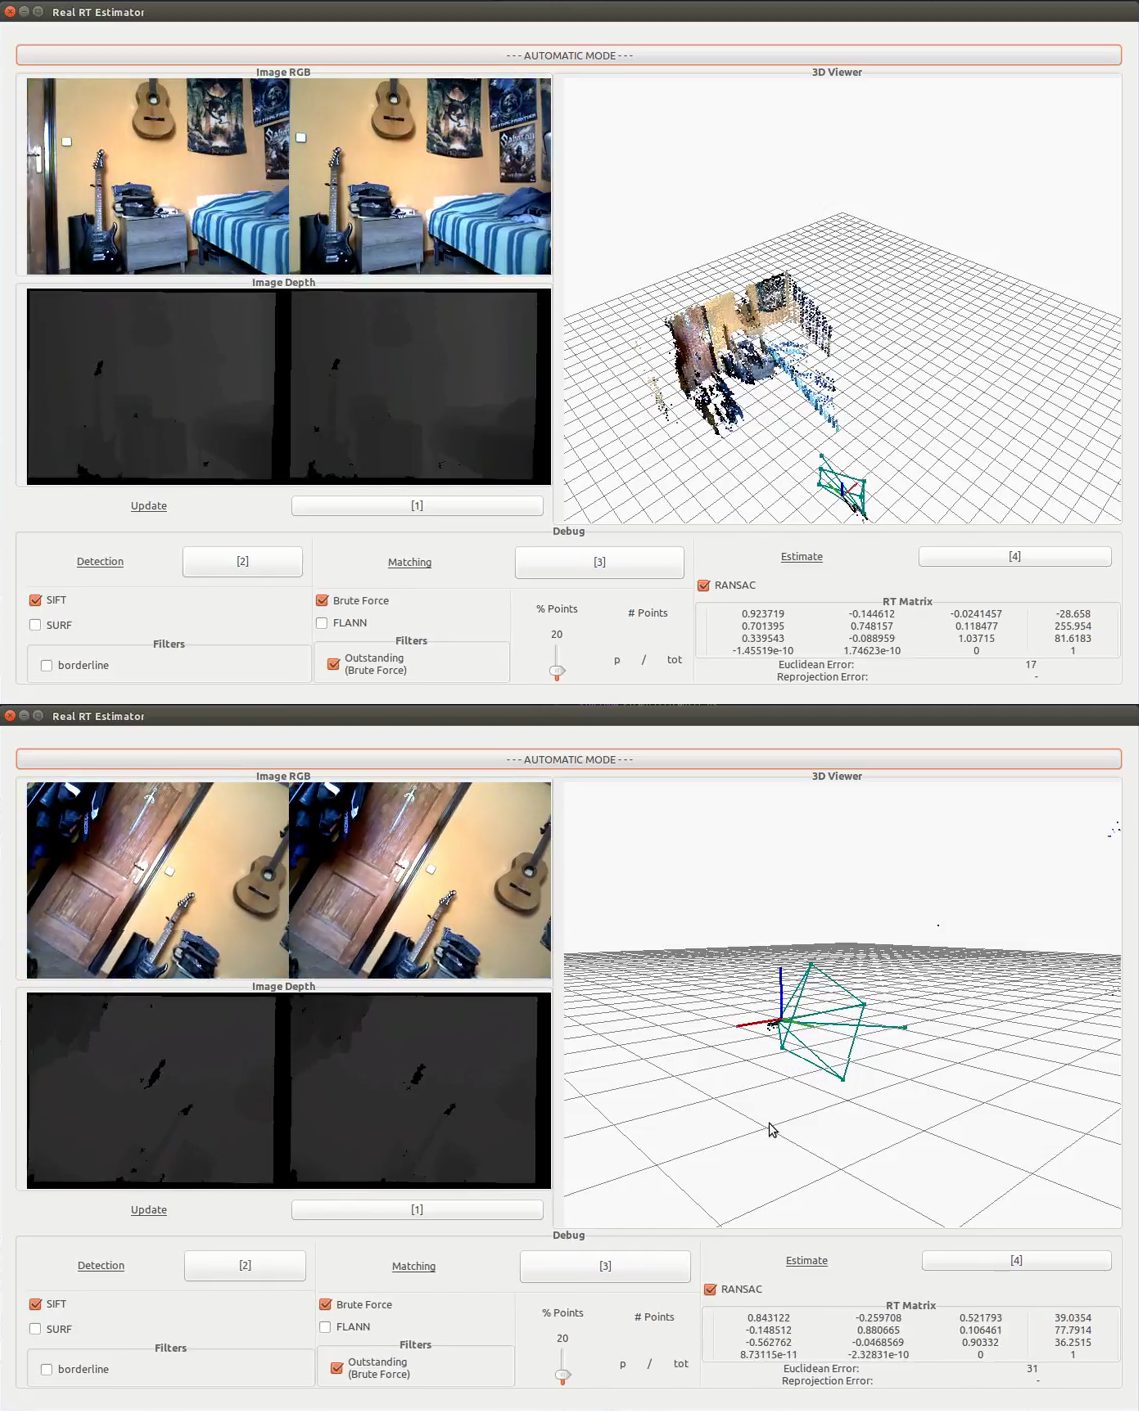
\includegraphics[scale=0.3]{Figures/tests/yaw-roll.png}
\decoRule
\caption[Pruebas con desplazamiento en los angulos \textit{yaw} y \textit{roll}]{Pruebas con desplazamiento en los angulos \textit{yaw} y \textit{roll}.}
\label{fig:yaw-roll}
\end{figure}

\subsubsection{Validación de trayectorias complejas}

\subsection{Error estático}

El error estático muestra el ruido blanco que se esconde detrás de la resolución 3D en tiempo real. Como se va a poder observar en esta sección, el ruido estático es inevitable y no depende del algoritmo a utilizar. Sin embargo, en el siguiente capítulo, en el cual se propone posibles mejoras y líneas futuras, se verán métodos para poder elimnarlo en mayor o menor medida.

En las siguientes Figura~\ref{fig:static} se puede ver un ejemplo de este error para diferentes configuraciones. Como se puede interpretar es un error que está presente en todos los casos.

\begin{figure}[th]
\centering
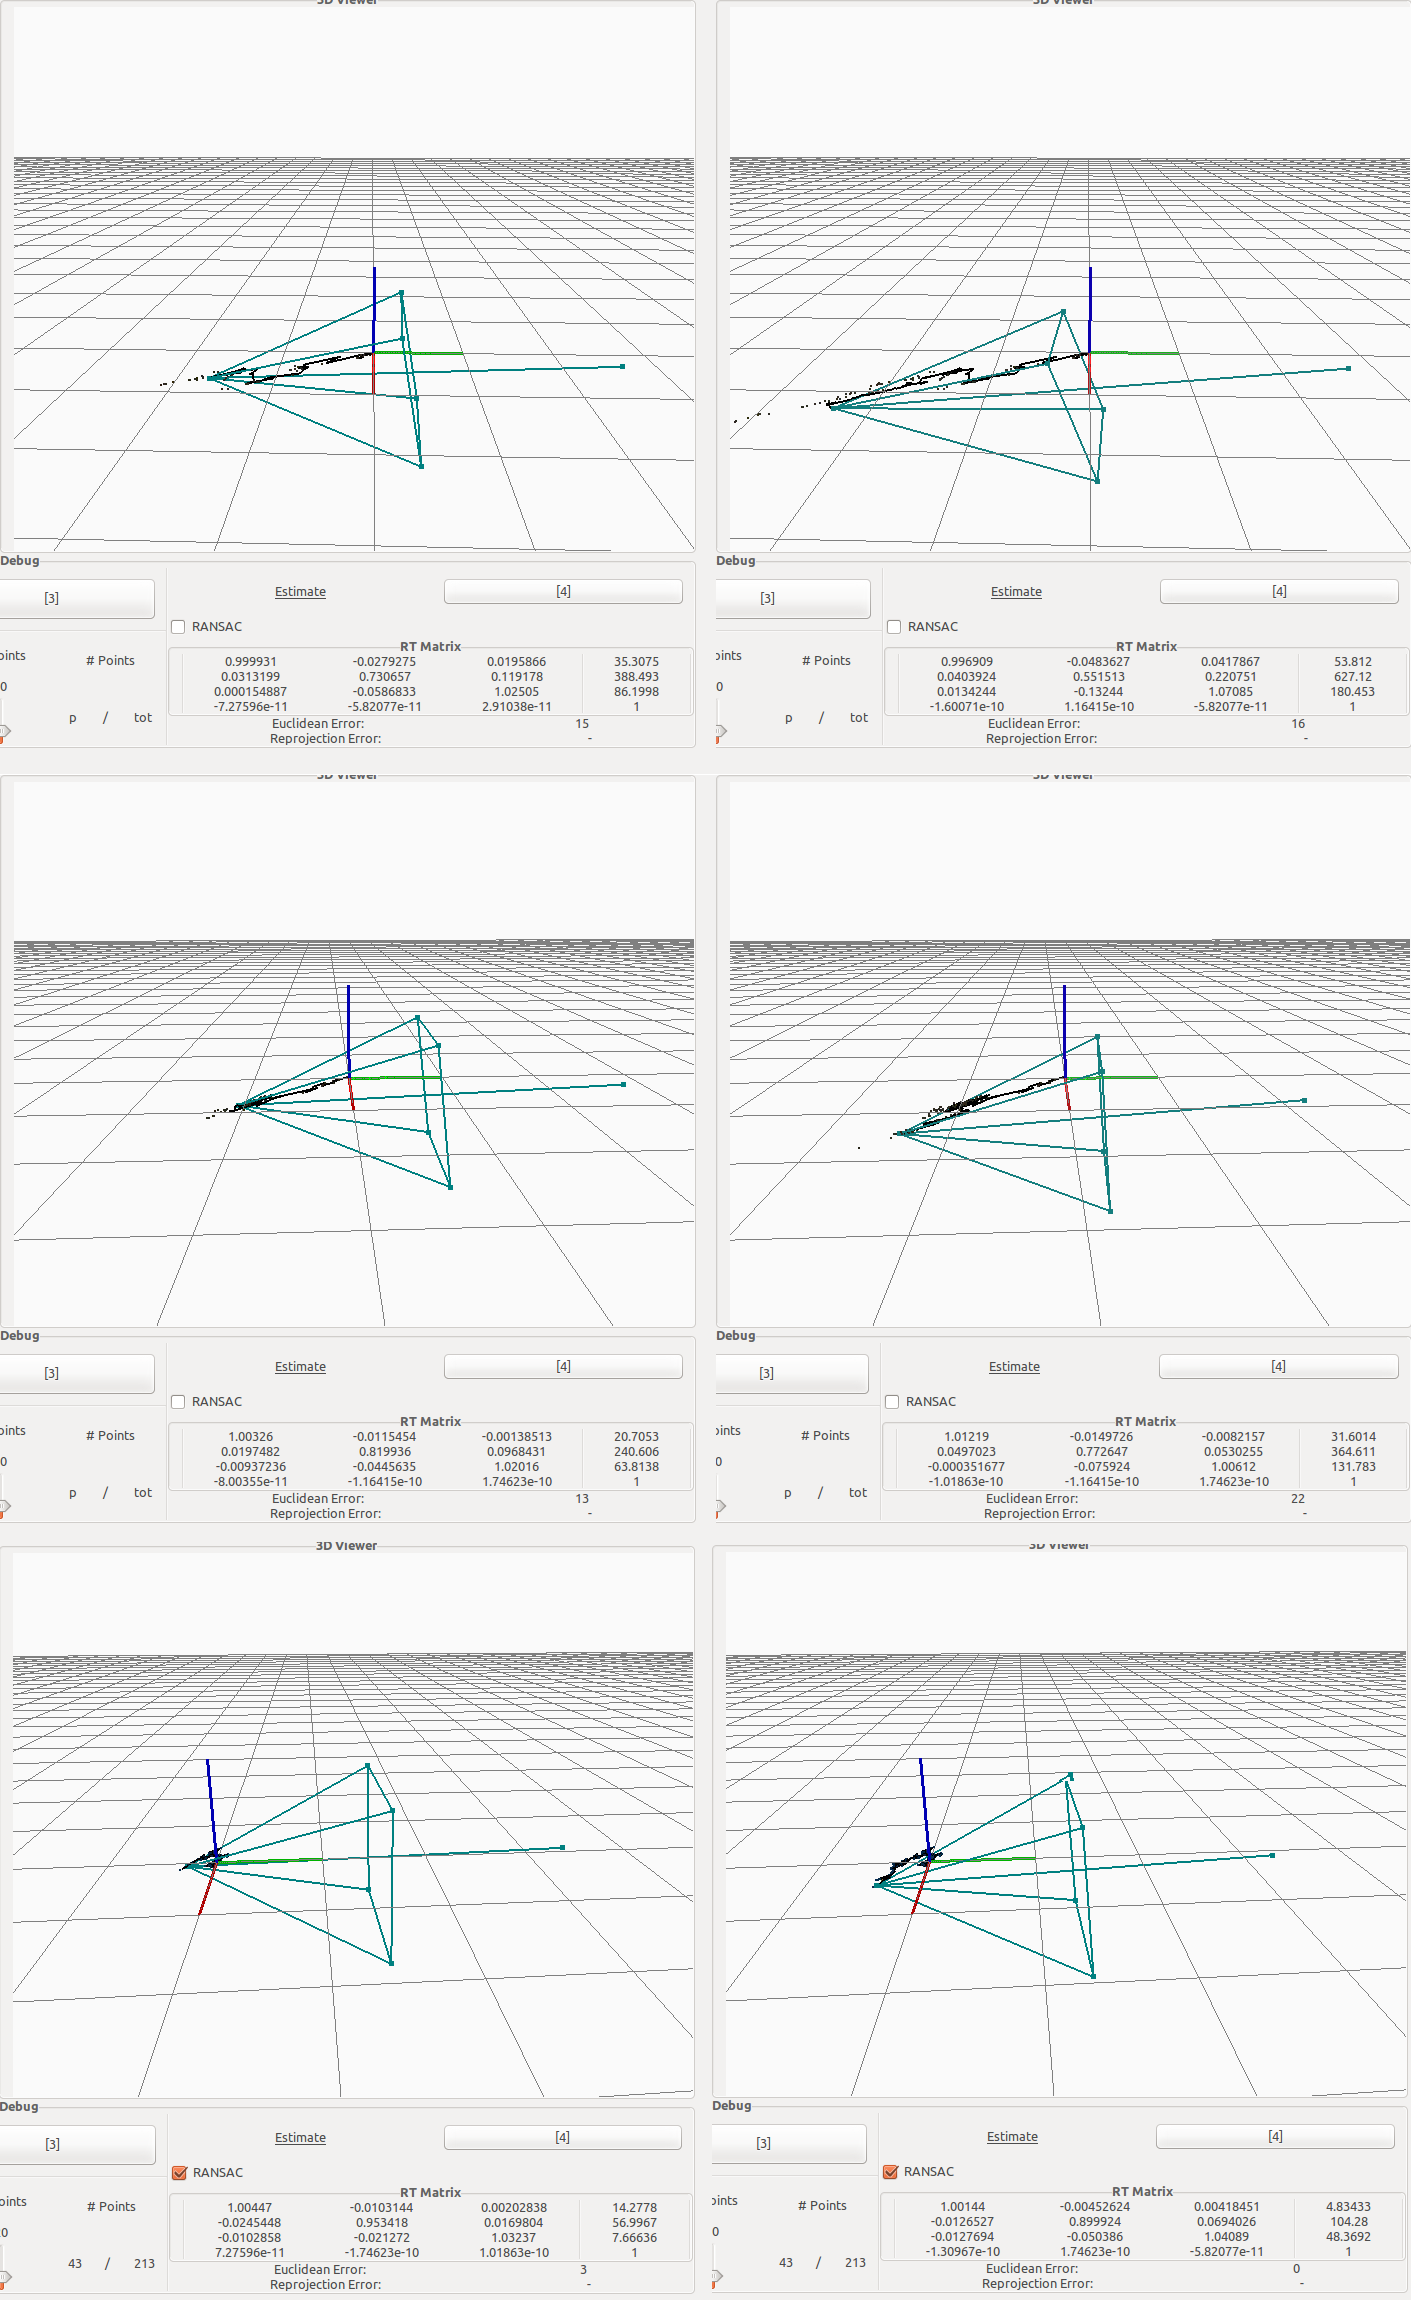
\includegraphics[scale=0.3]{Figures/tests/static.png}
\decoRule
\caption[Capturas con ruido estático]{En la primera imágen se representa el ruido estático después de 30 y 60 segundos, con SURF y FLANN. La segunda con SIFT, Fuerza Bruta y filtros. La tercera con SIFT, Fuerza Bruta y RANSAC.}
\label{fig:static}
\end{figure}

%\begin{figure}[th]
%\centering
%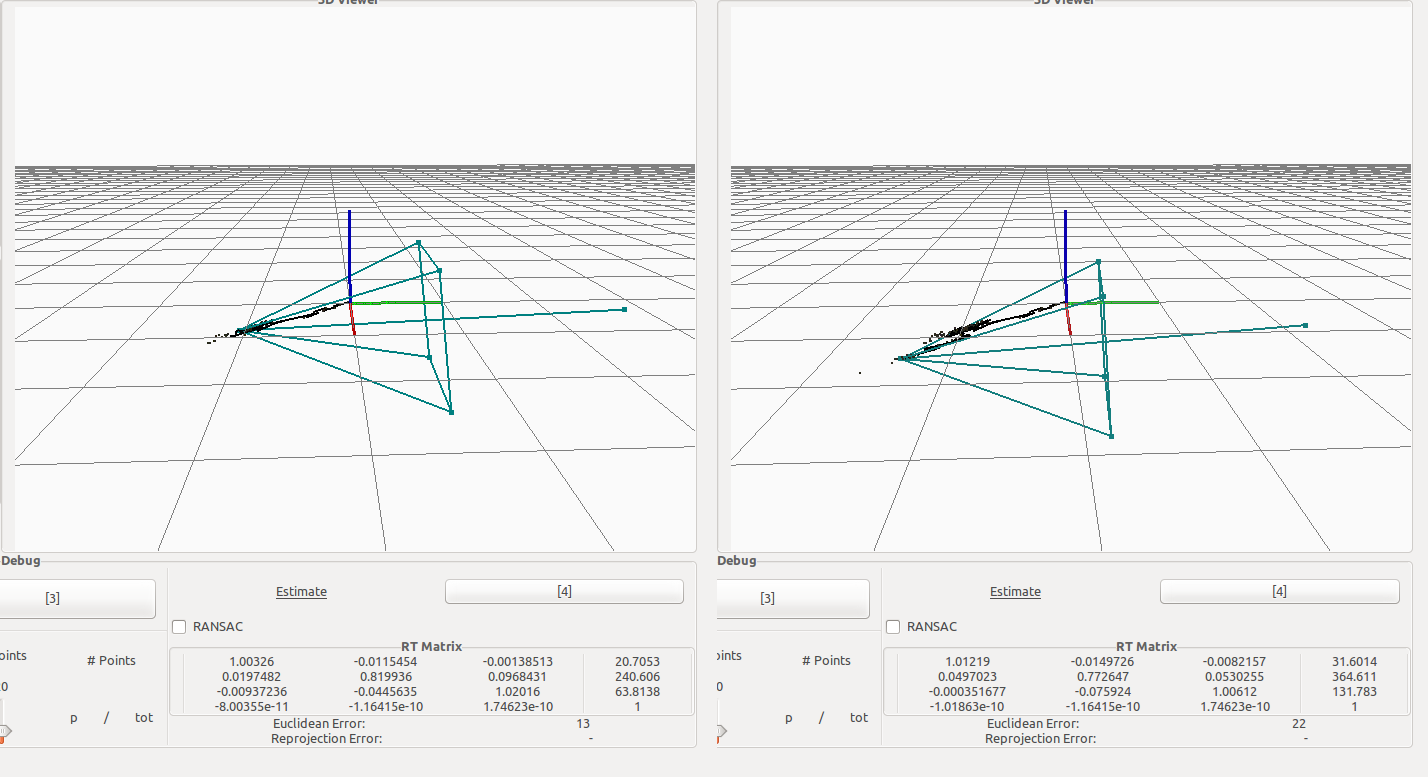
\includegraphics[scale=0.3]{Figures/tests/static-filter_2.png}
%\decoRule
%\caption[Ruido estático, con SIFT, Fuerza Bruta y filtros]{Ruido estático después de 30 y 60 segundos, con SIFT, Fuerza Bruta y filtros.}
%\label{fig:static2}
%\end{figure}
%
%\begin{figure}[th]
%\centering
%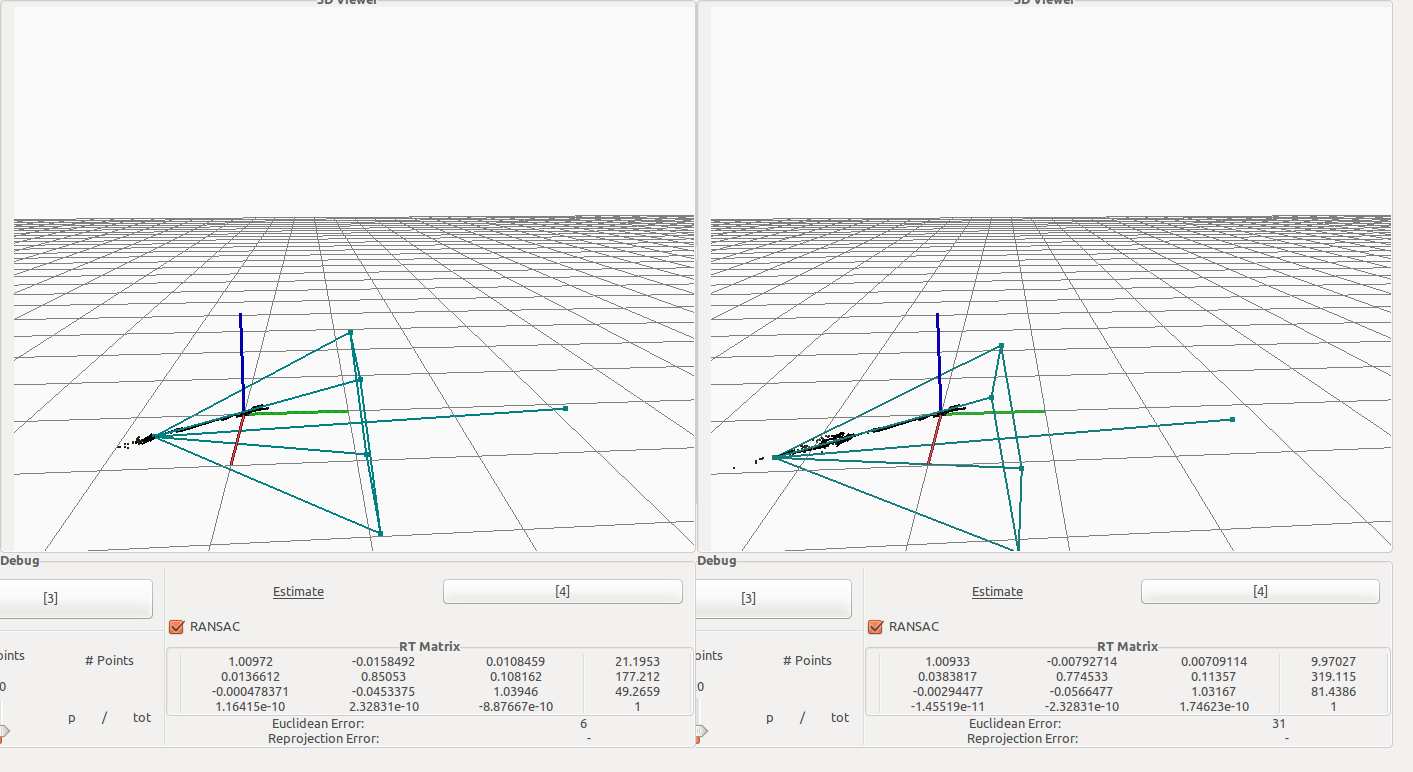
\includegraphics[scale=0.3]{Figures/tests/static-ransac_2.png}
%\decoRule
%\caption[Ruido estático, con SIFT, Fuerza Bruta y RANSAC]{Ruido estático después de 30 y 60 segundos, con SIFT, Fuerza Bruta y RANSAC.}
%\label{fig:static3}
%\end{figure}

Las pruebas realizadas han sido capturadas a los 30 y 60 segundos respectivamente y la configuración aplicada se encuentra en la descripción de cada Figura.

Si analizamos las matrices RT obtenidas se puede observar que el eje en que más avanza el ruido es el eje $y$, al igual que pasaba en las pruebas de la sección anterior.


%-----------------------------------
%	SECTION Tiempos de procesado
%-----------------------------------
\newpage
\section{Tiempos de procesado}
En esta sección se verán los tiempos de procesado del componente realizado en este proyecto. Como el componente realiza distintas tareas hasta completar una iteración completa, se ha desarrollado una funcionalidad que mide el tiempo medio por cada una de ellas cuando se termina la ejecución del componente.

Se irá analizando el tiempo medio para diferentes configuraciones en un intervalo de 10 segundos. Para un uso por defecto de la aplicación, se tiene:

\begin{lstlisting}[style=CStyle]
Average times:
- Update images: 0.678057 ms
- Points detection: 134.506 ms
- Points matching: 14.0233 ms
- Estimate matrix: 2.5231 ms
-----------------------------
- TOTAL: 151.731 ms
\end{lstlisting}

Como se puede observar la detección de puntos es la parte que más tiempo requiere, por el contrario, la estimación de la matriz RT es la que menos. Esta prueba se ha realizado con una media de unos 300 puntos de interés por iteración. Como es lógico el tiempo de detección variará con respecto al número de puntos de interés o carácterísticas extraídas. Estos puntos de interés según las pruebas no solo están condicionadas a la imágen que se está analizando, si no que la intensidad de luz desempeña un papel muy importante en la extracción de más o menos características.

En la siguiente tabla podemos ver la variabilidad de tiempo de detección para diferentes números de puntos:

\begin{table}
\caption{Tiempos medios de detección en relación a los puntos de interés}
\label{tab:detection-time}
\centering
\begin{tabular}{ l | l }
\toprule
\textbf{Número de puntos} & \textbf{Tiempo (ms)}\\
\hline\hline
100 & 102.27\\
\hline
200 & 117.136\\
\hline
250 & 126.019\\
\hline
300 & 134.506\\
\hline
350 & 137.805\\
\hline
400 & 144.408\\
\bottomrule
\end{tabular}
\end{table}

En esta etapa se ha incluído además el cálculo de 
